\documentclass[11pt]{article}

\usepackage{graphicx}
\usepackage{amsfonts}
\usepackage{amsmath}
\usepackage{amsthm}
\usepackage{latexsym}
\usepackage{amssymb}

\newtheorem{theorem}{Theorem}[section]
\newtheorem{lemma}[theorem]{Lemma}
\newtheorem{corollary}[theorem]{Corollary}
\newtheorem{assumption}[theorem]{Assumption}
\newtheorem{proposition}[theorem]{Proposition}
\newtheorem{observation}[theorem]{Observation}
\newtheorem{defin}[theorem]{Definition}
\newtheorem{definition}[theorem]{Definition}
\newtheorem{example}[theorem]{Example}
\newtheorem{conjecture}[theorem]{Conjecture}
\newtheorem{claim}{Claim}

\pagestyle{plain}
\bibliographystyle{plain}

\title{dfghdsgh}
\author{}

\begin{document}

\maketitle

\section{Introduction}

Clustering can be considered the most important unsupervised learning problem; so, as every other problem of this kind, it deals with finding a structure in a collection of unlabeled data.
A loose definition of clustering could be “the process of organizing objects into groups whose members are similar in some way”.
A cluster is therefore a collection of objects which are “similar” between them and are “dissimilar” to the objects belonging to other clusters.
We can show this with a simple graphical example:

\begin{figure}
\begin{center}
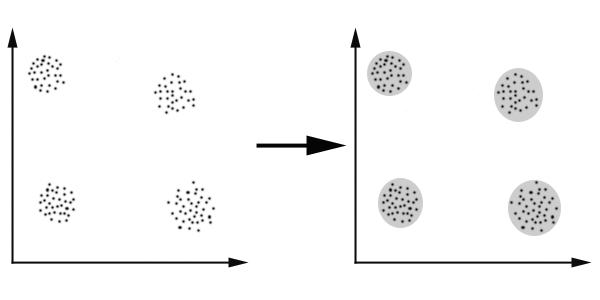
\includegraphics[scale=0.3]{clustering.jpg}
\end{center}

\end{figure}




\end{document}
